% PDFLaTeX
\documentclass[a4paper,12pt,twoside,spanish]{amsbook}

\input{tareas_definiciones} 


\begin{document}

\tarea{10}

\begin{ejercicio}[1] (40 pts) Determinar si el grafo $G=(V, E)$ tiene caminatas o circuitos eulerianos y  en caso de que la respuesta sea positiva encontrar una caminata o circuito euleriano. 

\begin{align*}
    V &= \{a, b, c, d, e, f, g, x, y, z, v, w\},\\
    E &= \{\{a, d\},
    \{b, d\},
    \{c, d\}, 
    \{d, e\},
    \{e, y\}, 
    \{f, w\},
    \{f, v\},
    \{g, x\}, 
    \\
    &\qquad\qquad\qquad\qquad\qquad\qquad\qquad\qquad
    \{g, y\},
    \{v, w\}, 
    \{v, y\}, 
    \{v, z\}, 
    \{y, z\}\}.
\end{align*}
\end{ejercicio}

\begin{ejercicio}[2]
    Dados los siguientes grafos:
\vskip .2cm

\begin{center}
    (1)\begin{tikzpicture}[scale=0.7]
        %\SetVertexSimple[Shape=circle,FillColor=white]
        \def\rvar{1.2}
        \Vertex[x=0.00, y=-0.00, L=$c$]{$u$} % 3
        \Vertex[x=\rvar*1.90, y=-0.62, L=$e$]{$t$} % 2
        \Vertex[x=\rvar*1.18, y=1.62, L=$b$]{$q$} % 1
        \Vertex[x=-1.18*\rvar, y=1.62, L=$a$]{$p$} % 0
        \Vertex[x=-1.90*\rvar, y=-0.62, L=$d$]{$r$} % 4
        \Vertex[x=0.00, y=-2.00, L=$f$]{$s$} % 5
        \Edges($u$,$t$,$q$,$p$)
        \Edges($r$,$u$)
        \Edges($s$,$t$)
        \Edges($r$,$s$,$q$,$r$)
        \Edges($p$,$t$,$s$)
        \Edges($s$,$p$,$r$)
    \end{tikzpicture}\quad\quad
    (2)\begin{tikzpicture}[scale=0.7]
        %\SetVertexSimple[Shape=circle,FillColor=white]
        \Vertex[x=-1.2, y=2, L=$p$]{$p$} % 0
        \Vertex[x= 1.2, y=2, L=$q$]{$q$} % 1
        \Vertex[x=-2, y=-0.0, L=$r$]{$r$} % 2
        \Vertex[x=-1.2, y=-2, L=$s$]{$s$} % 3
        \Vertex[x=2, y=-0.0, L=$t$]{$t$} % 4
        \Vertex[x= 1.2, y=-2, L=$u$]{$u$} % 5
        \Edges($s$,$r$,$p$,$q$,$r$,$u$,$t$,$p$,$s$,$q$)
    \end{tikzpicture}\quad\quad
    (3)\begin{tikzpicture}[scale=0.7]
        %\SetVertexSimple[Shape=circle,FillColor=white]
        \def\rvar{1.2}
        \Vertex[x=-1.18*\rvar, y=1.62, L=$4$]{$p$} % 0
        \Vertex[x=\rvar*1.18, y=1.62, L=$3$]{$q$} % 1
        \Vertex[x=-1.90*\rvar, y=-0.62, L=$5$]{$r$} % 2
        \Vertex[x=0, y=0, L=$6$]{$s$} % 3
        \Vertex[x=\rvar*1.90, y=-0.62, L=$2$]{$t$} % 4
        \Vertex[x=0.00, y=-2.00, L=$1$]{$u$} % 5
        
        
        
        \Edges($s$,$r$,$p$,$q$,$r$,$u$,$t$,$p$,$s$,$q$)
    \end{tikzpicture}
\end{center}
\vskip .3cm
\begin{enumerate}
        \item[(a)]  (20 pts) Dé un {ciclo hamiltoniano} en el grafo (1).
        \item[(b)]  (40 pts) Determinar cuales de los siguientes pares de grafos son isomorfos. En el caso de ser isomorfos, especifique un isomorfismo;
        en caso contrario, justificar por que no son isomorfos.

        (i) (1) y (2).\quad % no son isomorfos,(2) tiene una valencia 3, (1) no 

        (ii) (2) y (3). % Son isomorfos: p->4, q->3, r->5, s->6, t->2, u->1  
        % 
	\end{enumerate}
\end{ejercicio}
\vskip .2cm
\begin{comment}

\noindent{\color{blue}Solución.}




\end{comment}
\end{document}

